%!TEX root=../protocol.tex	% Optional

\section{Popis měřeného předmětu}
Devítisvorkový přípravek na vytváření signálů různých šířek a průběhů.

\section{Teoretický rozbor}
Pro začátek je důležité zmínit, že osciloskop, analogový i digitální, je pouze zobrazovací přístroj, a tedy \glqq{}naměřená\grqq{} data se nedají považovat za správné, či dokonce přesné.
\\\\
$V_{pp}$, celým názvem Voltage Peak to Peak, je rozdíl největšího a nejmenšího napětí. Visuálně na osciloskopu je to vertikální rozsah mezi nejvyšším a nejnižším bodem vlny.
\\
\[V_{pp} = U_{Max} - U_{Min} \]
\\\\
Střední hodnota střídavého napětí $U_{Avg}$ je taková hodnota stejnosměrného napětí, která má stejné nábojové účinky jako měřené střídavé napětí. Jedná se o průměrnou hodnotu za periodu (často i za půl periodu).
\\
Pro nestřídavé napětí (například konstantní zdroj napětí) je střední hodnota pak jednoduše rovna samotné hodnotě napětí.
\\
\[U_{Avg} = \int_0^T U dt \] kde T je perioda měřeného napětí.
\\\\
Efektivní hodnota napětí $U_{RMS}$ (RMS = Root Mean Square) je taková hodnota stejnosměrného napětí, která má stejné energetické účinky jako měřené střídavé napětí. Určuje se z průměrného výkonu za periodu.
\\


\section{Postup měření}
Pomocí měřících sond nastavených v poměru 1:1 se připojí sledovaný signál k osciloskopu. Po nastavení zobrazení signálu se všechna měření prováděla v menu osciloskopu, podle zadání.

\newpage
\section{Naměřené hodnoty}

\begin{table}[h!]

\captionsetup{justification=raggedright,singlelinecheck=false, margin={1.5cm,0cm}} % Move caption to the left
\caption{Změřené hodnoty při plnění jednotlivých bodů zadání}
\centering
\begin{tabular}{ | c | c | } 
  \hline
  Měřená veličina & hodnota \\ 
  \hline
  frekvence &  1,953 kHz\\ 
  \hline
  perioda  &  512,03 µs\\ 
  \hline
  $U_{RMS}$ & 2,35 V \\ 
  \hline
  $U_{Avg}$ & 1,66 V \\ 
  \hline
  $V_{pp}$ &  3,50 V\\ 
  \hline
  Hold Off time & 9,1 ms \\ 
  \hline
  Glitch time   & 1,00 µs \\ 
  \hline
  Time (falling - falling) & 1,28 ms \\ 
  \hline
  Time (rising - rising)   & 255,9 µs \\ 
  \hline
  Runt Low  & 2,8 V \\ 
  \hline
  Runt High   & 3,9 V \\ 
  \hline
  Rising Edge time & 3,8 ns \\ 
  \hline
  
\end{tabular}
\label{table:2}
\end{table}

\begin{table}[h!]

\captionsetup{justification=raggedright,singlelinecheck=false, margin={1.5cm,0cm}} % Move caption to the left
\caption{Změřené hodnoty pro DC mód}
\centering
\begin{tabular}{ | c | c | } 
  \hline
  Měřená veličina & hodnota \\ 
  \hline
  frekvence &  1,953 kHz\\ 
  \hline
  perioda  &  512,03 µs\\ 
  \hline
  $U_{RMS}$ & 2,35 V \\ 
  \hline
  $U_{Avg}$ & 1,66 V \\ 
  \hline
  $V_{pp}$ &  3,50 V\\ 
  \hline
  
\end{tabular}
\label{table:3}
\end{table}

\begin{table}[h!]

\captionsetup{justification=raggedright,singlelinecheck=false, margin={1.5cm,0cm}} % Move caption to the left
\caption{Změřené hodnoty pro AC mód}
\centering
\begin{tabular}{ | c | c | } 
  \hline
  Měřená veličina & hodnota \\ 
  \hline
  frekvence &  1,953 kHz\\ 
  \hline
  perioda  &  512,03 µs\\
  \hline
  $U_{RMS}$ & 1,5 V \\ 
  \hline
  $U_{Avg}$ & 120 mV \\ 
  \hline
  $V_{pp}$ &  3,60 V\\ 
  \hline
  
\end{tabular}
\label{table:4}
\end{table}

V režimu \textbf{Single}: Rising slope 160 µs, Falling slope 155 µs.
\\
\newpage

\begin{figure}[h]
\centering
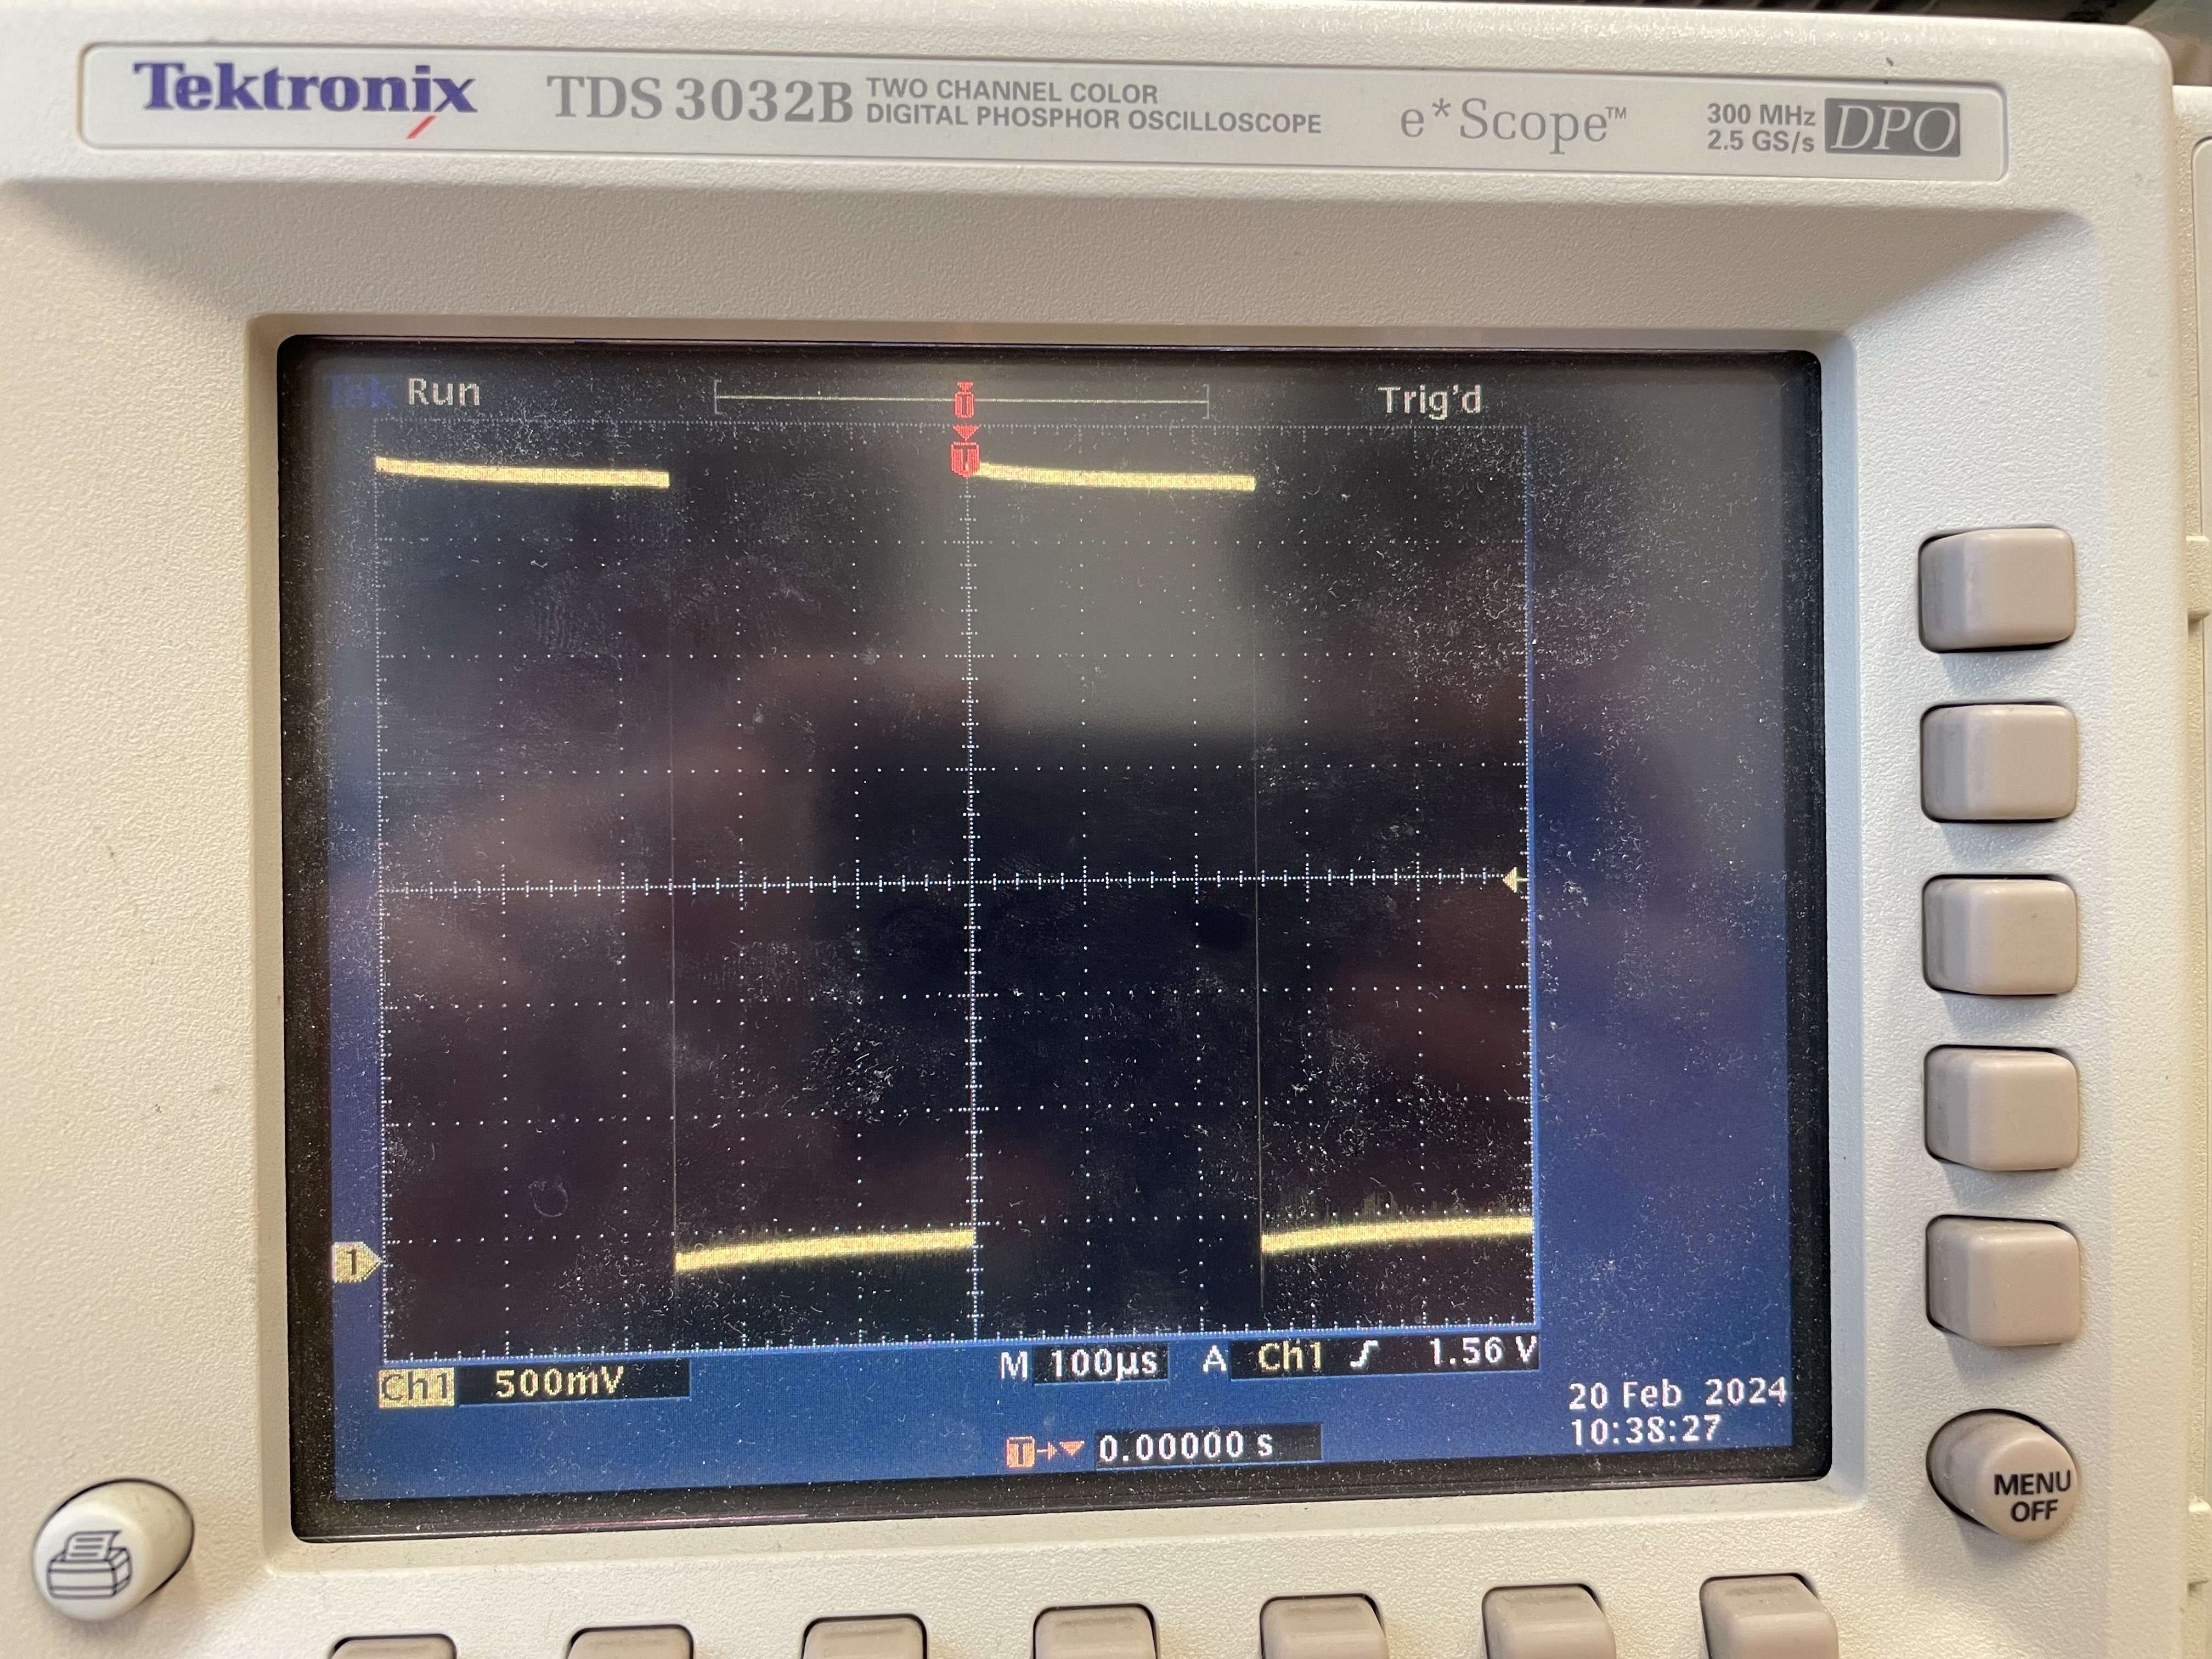
\includegraphics[width=12cm]{images/mereni-1.jpg}
\caption{Fotka řešení zadání 1.1}
\label{fig:1}
\end{figure}


\section{Zhodnocení}
Pro synchronizování signálu jsme Hold-off dobu stanovili pro dvě periody signálu. Maximální a minimální šířku pulsu jsme vybrali takovým způsobem, aby Glitch byl patrný v posledním pulsu.
